% Template LaTeX file for LAC-20 papers
%
% To generate the correct references using BibTeX, run
%     latex, bibtex, latex, latex
% modified...
% - from DAFx-00 to DAFx-02 by Florian Keiler, 2002-07-08
% - from DAFx-02 to DAFx-03 by Gianpaolo Evangelista
% - from DAFx-05 to DAFx-06 by Vincent Verfaille, 2006-02-05
% - from DAFx-06 to DAFx-07 by Vincent Verfaille, 2007-01-05
%                          and Sylvain Marchand, 2007-01-31
% - from DAFx-07 to DAFx-08 by Henri Penttinen, 2007-12-12
%                          and Jyri Pakarinen 2008-01-28
% - from DAFx-08 to DAFx-09 by Giorgio Prandi, Fabio Antonacci 2008-10-03
% - from DAFx-09 to DAFx-10 by Hannes Pomberger 2010-02-01
% - from DAFx-10 to DAFx-12 by Jez Wells 2011
% - from DAFx-12 to DAFx-14 by Sascha Disch 2013
% - from DAFx-15 to DAFx-16 by Pavel Rajmic 2015
% - from DAFx-16 to IFC-18 by Romain Michon 2018
% - from IFC-18 to LAC-19 by Romain Michon 2019
% - from LAC-19 to LAC-20 by Jean-Michaël Celerier 2020
%
% Template with hyper-references (links) active after conversion to pdf
% (with the distiller) or if compiled with pdflatex.
%
% 20060205: added package 'hypcap' to correct hyperlinks to figures and tables
%                      use of \papertitle and \paperauthorA, etc for same title in PDF and Metadata
%
% 1) Please compile using lualatex, latex or pdflatex.
% 2) If using pdflatex, you need your figures in a file format other than eps! e.g. png or jpg is working
% 3) Please use "papertitle" and "pdfauthor" definitions below

%------------------------------------------------------------------------------------------
%  !  !  !  !  !  !  !  !  !  !  !  ! user defined variables  !  !  !  !  !  !  !  !  !  !  !  !  !  !
% Please use these commands to define title and author(s) of the paper:
\def\papertitle{SEAM PROJECT - Sustained Electroacoustic Music}
\def\paperauthorA{Davide Tedesco}
\def\paperauthorB{Giuseppe Silvi}
%\def\paperauthorC{Author Three}
%\def\paperauthorD{Author Four}

% Authors' affiliations have to be set below

%------------------------------------------------------------------------------------------
\documentclass[twoside,a4paper]{article}
\usepackage{LAC-20}
\usepackage{amsmath,amssymb,amsfonts,amsthm}
\usepackage{euscript}
\usepackage{ifpdf}
\usepackage{ifluatex}
\usepackage{ifxetex}

\usepackage{color}
\usepackage{listings}
\definecolor{mygrey}{rgb}{0.96,0.96,0.96}
\lstset{
  tabsize=4,
  basicstyle=\ttfamily,
  backgroundcolor=\color{mygrey},
  captionpos=b,
  breaklines=true
}

\usepackage[english]{babel}
\usepackage{caption}
\usepackage{subfig, color}
\setcounter{page}{1}
\ninept

\usepackage{times}
% pdf-tex settings: detect automatically if run by latex or pdflatex
\ifluatex
  \usepackage[
    pdftitle={\papertitle},
    pdfauthor={\paperauthorA, \paperauthorB},%, \paperauthorC, \paperauthorD},
    colorlinks=false, % links are activated as colror boxes instead of color text
    bookmarksnumbered, % use section numbers with bookmarks
    pdfstartview=XYZ % start with zoom=100% instead of full screen; especially useful if working with a big screen :-)
  ]{hyperref}
  
  \edef\pdfcompresslevel{\pdfvariable compresslevel}
  \pdfcompresslevel=9
  \usepackage{graphicx}
  
  \usepackage[figure,table]{hypcap}
  \usepackage{fontspec}
\else
  \ifxetex
    \usepackage[
      pdftitle={\papertitle},
      pdfauthor={\paperauthorA, \paperauthorB},%, \paperauthorC, \paperauthorD},
      colorlinks=false, % links are activated as colror boxes instead of color text
      bookmarksnumbered, % use section numbers with bookmarks
      pdfstartview=XYZ % start with zoom=100% instead of full screen; especially useful if working with a big screen :-)
    ]{hyperref}
    
    \pdfcompresslevel=9
    \usepackage{graphicx}
    
    \usepackage[figure,table]{hypcap}
    \usepackage{fontspec}
  \else
    \usepackage[utf8]{inputenc}
    \usepackage[T1]{fontenc}
    \ifpdf % compiling with pdflatex
      \usepackage[pdftex,
        pdftitle={\papertitle},
        pdfauthor={\paperauthorA, \paperauthorB},%, \paperauthorC, \paperauthorD},
        colorlinks=false, % links are activated as colror boxes instead of color text
        bookmarksnumbered, % use section numbers with bookmarks
        pdfstartview=XYZ % start with zoom=100% instead of full screen; especially useful if working with a big screen :-)
      ]{hyperref}
      \pdfcompresslevel=9
      \usepackage[pdftex]{graphicx}
      \usepackage[figure,table]{hypcap}
      \DeclareGraphicsExtensions{.png,.jpg,.pdf}
    \else % compiling with latex
      \usepackage[dvips]{epsfig,graphicx}
      \usepackage[dvips,
        colorlinks=false, % no color links
        bookmarksnumbered, % use section numbers with bookmarks
        pdfstartview=XYZ % start with zoom=100% instead of full screen
      ]{hyperref}
      % hyperrefs are active in the pdf file after conversion
      \usepackage[figure,table]{hypcap}
      \DeclareGraphicsExtensions{.eps}
    \fi
  \fi
\fi

\title{\papertitle}

%-------------SINGLE-AUTHOR HEADER STARTS (uncomment below if your paper has a single author)-----------------------
% \affiliation{
% \paperauthorA \,\sthanks{This work was supported by the XYZ Foundation}}
% {\href{https://scrime.u-bordeaux.fr}{SCRIME} \\ Université de Bordeaux, France \\
% {\tt \href{mailto:ping@linuxaudio.org}{ping@linuxaudio.org}}
% }
%-----------------------------------SINGLE-AUTHOR HEADER ENDS------------------------------------------------------

%---------------TWO-AUTHOR HEADER STARTS (uncomment below if your paper has two authors)-----------------------
 \twoaffiliations{
 \paperauthorA \,\sthanks{This work was supported by the XYZ Foundation}}
 {\href{https://scrime.u-bordeaux.fr}{SCRIME} \\ Université de Bordeaux, France \\
 {\tt \href{mailto:ping@linuxaudio.org}{ping@linuxaudio.org}}
 }
 {\paperauthorB \,\sthanks{This guy is a very good fellow}}
 {\href{https://ccrma.stanford.edu}{CCRMA} \\ Stanford University, USA \\
 {\tt \href{mailto:lac@ccrma.stanford.edu}{lac@ccrma.stanford.edu}}
 }
%-------------------------------------TWO-AUTHOR HEADER ENDS------------------------------------------------------

%---------------THREE-AUTHOR HEADER STARTS (uncomment below if your paper has three authors)-----------------------
% \threeaffiliations{
% \paperauthorA \,\sthanks{This work was supported by the XYZ Foundation}}
% {\href{https://scrime.u-bordeaux.fr}{SCRIME} \\ Université de Bordeaux, France \\
% {\tt \href{mailto:ping@linuxaudio.org}{ping@linuxaudio.org}}
% }
% {\paperauthorB \,\sthanks{This guy is a very good fellow}}
% {\href{https://ccrma.stanford.edu}{CCRMA} \\ Stanford University, USA \\
% {\tt \href{mailto:lac@ccrma.stanford.edu}{lac@ccrma.stanford.edu}}
% }
% {\paperauthorC \,\sthanks{Illustrious contributor}}
% {\href{http://www.musikwissenschaft.uni-mainz.de/Musikinformatik/}{Johannes Gutenberg University (JGU)} \\  Mainz, Germany\\
% {\tt \href{mailto:lac@uni-mainz.de}{lac@uni-mainz.de}}
% }
%-------------------------------------THREE-AUTHOR HEADER ENDS------------------------------------------------------

%----------------FOUR-AUTHOR HEADER STARTS (uncomment below if your paper has four authors)-----------------------
%\fouraffiliations{
%\paperauthorA \,\sthanks{This work was supported by the XYZ Foundation}}
%{\href{https://scrime.u-bordeaux.fr}{SCRIME} \\ Université de Bordeaux, France \\
%{\tt \href{mailto:ping@linuxaudio.org}{ping@linuxaudio.org}}
%}
%{\paperauthorB \,\sthanks{This guy is a very good fellow}}
%{\href{https://ccrma.stanford.edu}{CCRMA} \\ Stanford University, USA \\
%{\tt \href{mailto:lac@ccrma.stanford.edu}{lac@ccrma.stanford.edu}}
%}
%{\paperauthorC \,\sthanks{Illustrious contributor}}
%{\href{http://www.musikwissenschaft.uni-mainz.de/Musikinformatik/}{Johannes Gutenberg University (JGU)} \\  Mainz, Germany\\
%{\tt \href{mailto:lac@uni-mainz.de}{lac@uni-mainz.de}}
%}
%{\paperauthorD \,\sthanks{Thanks to the predecessors for the templates}}
%{\href{https://c-base.org/}{C-Base} \\ Berlin, Germany \\
%{\tt \href{mailto:lac@c-base.com}{lac@c-base.com}}
%}
%-------------------------------------FOUR-AUTHOR HEADER ENDS------------------------------------------------------

\begin{document}

\maketitle

\begin{abstract}
This is the template file for the proceedings of the 18$^{\text{th}}$ 
Linux Audio Conference (LAC-20).
This template has been derived from DAFx-16, IFC-18, LAC-19 templates and aims at 
producing conference proceedings in electronic form.
The format is essentially the one used for ICASSP conferences. Please use
either this \LaTeX{} or the accompanying LibreOffice formats when preparing your
submission. 
\end{abstract}

\section{Introduction}
\label{sec:intro}

This template can be found on the conference website.

\subsection{Figures}
\label{ssec:figures}

Sustained Electroacoustic Music is a project inspired by Alvise Vidolin and
Nicola Bernardini's article on electroacoustic music sustainability. In the
article, they point at multiple faces of the problem: technological, notational
or simple conceivement issue. They focus only on live electroacoustic music but
it is applicable to any kind of documented electroacoustic music.

The purpose of this project is to grow the interpretation and the electroacoustic
musical practice without electronics and informatics problems that obstacles the
approach to this music.

When we refer to a virtuoso musician often we point to a violinist or a piano player.
Someone who intensely practice on his instruments. This is the point: Does the
violinist build his own violin every time he approaches a new composition?
Does the pianist? The electroacoustic does.

The electroacoustic music culture was born in a daily changing contest. The
sustainability of what they were doing during the years wasn't a point for decades.
Actually, today neither. Not to the community. Sustainability is a complicated
concept at all. Music sustainability is something like an abstract problem applied
to an abstract thing only for a small number of people, like an abstract community
not related to the mass. (si sa che) Mass-media, mass-culture, are not place for the 
*sustained* people.

So we are speaking about a small problem in music culture. A small problem not for
mankind. But it is a problem. If the actual occidental music is or not afflicted
by the contemporary and electroacoustic music issues is a good question, but that
the music thinking was changed by electroacoustic thinking is a fact. Generally,
we can consider that music was changed inexorably after the introduction of
electronics and informatics in composition, playing and production.

Here are the points. What will happen when all the people who manipulates those
problems will disappear? What is the electroacoustic repertoire if it is not the
music played in the concert hall? Why we concentrate too many resources on
technics problems and not to musical interpretations and playing practice?

We can simply look at the Doctoral offers all over the world. There are so many
interactive-all-you-can-think-about. The music industry conceived the purpose of
doing music. With or without problems. During that interaction, during this art
of entertainment, where the industry is god, and god is a DJ, during this time
there is also a repertoire of music we must consider the core of the actual musical
thinking that will disappear in some years. Not the paper, neither the recordings.
Will disappear the practice, the interpretation, the thinking itself.

What will happen to the Luigi Nono's music after Alvise Vidolin? We have to study
Vidolin, to understand Nono, to have a see sight on our music through an era.

An example. We have three interpretations of Beethoven's Complete Symphonies, by
Karajan. Each of those boxsets is a thing, a collection of objects. Not music
itself. We have three sets of reproduction of the same musical things through the
same mind. Is a huge resources of thinking. Not a huge resource of music itself.
Every man who has listened to Beethoven in a concert hall knows perfectly that his
music can't fit in a box that can stay in a hand. But if the boxset is not
Beethoven's music itself, it sure is an object of thinking. There is a point, sure,
this is not the purpose it was built, but it doesn't matter.  The point is that
we have stratified musical thinking and listening attitude on Beethoven's music
through interpretations of his music. We have not rewritten his music each time.
We have not built his instruments each time. It is a technological fact? A musical
one too.

Luigi Nono's repertoire is not on a triple boxset of no one. It is on paper, in
the best of the case. We have some recordings, yes we have. What we can study and
interpret if half of the ensemble is Live Electronics Instruments dated the '80s
and it was not really described, not really sustained through the years?

What do we think about a lot of composers who have framed their music in events
without sustain at all their electronic instruments through the year?



All figures should be centered on the column (or page, if the figure spans both
columns). Figure captions (in italic) should follow each figure and have the
format given in Figure~\ref{fft_plot}. Vectorial figures are preferred (e.g.,
Postscript, PDF, etc.). Also, in order to provide a better readability, figure
text font size should be at least identical to footnote font size. If bitmap
figures are used, please make sure that the resolution is enough for print
quality. Figure~\ref{ftt_plot2} illustrates an example of a figure spanning two
columns.

\begin{figure}[ht]
\centerline{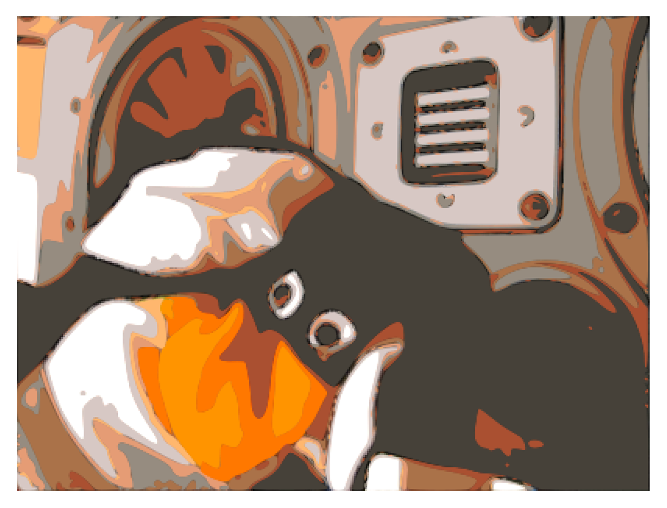
\includegraphics[scale=0.5]{ping}}
\caption{\label{fft_plot}{\it Ping.}}
\end{figure}

\begin{figure*}[ht]
\center
\includegraphics[width=5in]{TwoColumnSine2}
\caption{\label{ftt_plot2}{\it A figure spanning two columns, as mentioned in
Sec. \ref{ssec:figures}.}}
\end{figure*}

\subsection{Tables}

As for figures, all tables should be centered on the column (or page, if the
table spans both columns). Table captions should be in italic, precede each
table and have the format given in Table~\ref{tab:example}.

\begin{table}[ht]
  \caption{\itshape Basic trigonometric values.}
	\centering
	\begin{tabular}{|c|c|}
		\hline
		$\mathrm{angle}\,(\theta, \mathrm{rad})$ & $\sin \theta$ \\\hline
		$\frac{\pi}{2}$ & $1$ \\
		$\pi$ & $0$ \\
		$\frac{3\pi}{2}$ & $-1$ \\
		$2\pi$ & $0$ \\\hline
	\end{tabular}
	%
	\label{tab:example}
\end{table}

\begin{table*}[ht]
  \caption{{\it Basic trigonometric values, spanning two columns.}}
	\centering
  \begin{tabular}{|c|c|c|c|c|c|c|}\hline
    $\mathrm{angle}\, (\theta, \mathrm{rad})$ & $\sin \theta$ & $\cos \theta $ & $(\sin \theta)/2 $ & $(\cos \theta) /2 $ & $(\sin \theta)/3 $ & $(\cos \theta)/3$    \\\hline
    $\frac{\pi}{2}$ & $1$ & $0$ & $1/2$ & $0$ & $1/3$ & $0$ \\
    $\pi$ & $0$ & $-1$ & $0$ & $-1/2$ & $0$ & $-1/3$\\
    $\frac{3\pi}{2}$ & $-1$ & $0$ & $-1/2$ & $0$ & $-1/3$ & $0$ \\
    $2\pi$ & $0$ & $1$ & $0$ & $1/2$ & $0$ & $1/3$ \\\hline
 \end{tabular}
	%
  \label{tab:example2}
\end{table*}

\subsection{Equations}

Equations should be placed on separate lines and numbered:

\begin{equation}
	y(n)=b_0x(n)-a_1y(n-1)
	\label{eq1}
	\end{equation}
	where equation (\ref{eq1}) is a one pole filter with frequency response:
	\begin{equation}
	H(e^{j \omega T}) = \frac{b_0}{1+a_1e^{-j \omega T}}
	\label{eq2}
\end{equation}

\subsection{Code}

Code can be listed in a block:

\begin{lstlisting}
  int foo = 0;
\end{lstlisting}
\noindent
or directly in-lined in the body of the text: \lstinline{int foo = 1;}.

\subsection{Page Numbers}

Page numbers will be added to the document in the post-processing stage, so
{\em please leave the numbering as is} (no numbers).


\subsection{References}

The references will be numbered in order of appearance \cite{Sal89},
\cite{Spa72}, \cite{MosWal64} and \cite{Kay86}. Please avoid listing
references that do not appear in the text.

\subsubsection{Reference Format}

The reference format is the standard IEEE one. We recommend to use BibTeX to
create the reference list.

\section{Conclusions}

This template can be found on the conference website. For changing the number
of author affiliations (1 to 4), uncomment the corresponding regions in the
template \texttt{tex} file. Please, submit full-length papers (4 to 8 pages
for full papers and 2 to 4 pages for poster papers) and keep the paper size to
letter (don't change to A4). Submission is fully electronic and automated 
through the Conference Web Submission System. DO NOT send us papers directly by 
e-mail.

\section{Acknowledgments}

Many thanks to the great number of anonymous reviewers!

%\newpage
\nocite{*}
\bibliographystyle{IEEEbib}
\bibliography{LAC-20} % requires file lac-20.bib

\section{Appendix: Margin Check}

This section shows the column margins for the text.

Lorem ipsum dolor sit amet, consectetur adipisici elit, sed eiusmod tempor
incidunt ut labore et dolore magna aliqua. Ut enim ad minim veniam, quis
nostrud exercitation ullamco laboris nisi ut aliquid ex ea commodi consequat.
Quis aute iure reprehenderit in voluptate velit esse cillum dolore eu fugiat
nulla pariatur. Excepteur sint obcaecat cupiditat non proident, sunt in culpa
qui officia deserunt mollit anim id est laborum.

Duis autem vel eum iriure dolor in hendrerit in vulputate velit esse molestie
consequat, vel illum dolore eu feugiat nulla facilisis at vero eros et accumsan
et iusto odio dignissim qui blandit praesent luptatum zzril delenit augue duis
dolore te feugait nulla facilisi. Lorem ipsum dolor sit amet, consectetuer
adipiscing elit, sed diam nonummy nibh euismod tincidunt ut laoreet dolore
magna aliquam erat volutpat.

Ut wisi enim ad minim veniam, quis nostrud exerci tation ullamcorper suscipit
lobortis nisl ut aliquip ex ea commodo consequat. Duis autem vel eum iriure
dolor in hendrerit in vulputate velit esse molestie consequat, vel illum dolore
eu feugiat nulla facilisis at vero eros et accumsan et iusto odio dignissim qui
blandit praesent luptatum zzril delenit augue duis dolore te feugait nulla
facilisi.

Nam liber tempor cum soluta nobis eleifend option congue nihil imperdiet doming
id quod mazim placerat facer possim assum. Lorem ipsum dolor sit amet,
consectetuer adipiscing elit, sed diam nonummy nibh euismod tincidunt ut
laoreet dolore magna aliquam erat volutpat. Ut wisi enim ad minim veniam, quis
nostrud exerci tation ullamcorper suscipit lobortis nisl ut aliquip ex ea
commodo consequat.

Duis autem vel eum iriure dolor in hendrerit in vulputate velit esse molestie
consequat, vel illum dolore eu feugiat nulla facilisis.

At vero eos et accusam et justo duo dolores et ea rebum. Stet clita kasd
gubergren, no sea takimata sanctus est Lorem ipsum dolor sit amet. Lorem ipsum
dolor sit amet, consetetur sadipscing elitr, sed diam nonumy eirmod tempor
invidunt ut labore et dolore magna aliquyam erat, sed diam voluptua. At vero
eos et accusam et justo duo dolores et ea rebum. Stet clita kasd gubergren, no
sea takimata sanctus est Lorem ipsum dolor sit amet. Lorem ipsum dolor sit
amet, consetetur sadipscing elitr, At accusam aliquyam diam diam dolore dolores
duo eirmod eos erat, et nonumy sed tempor et et invidunt justo labore Stet
clita ea et gubergren, kasd magna no rebum. sanctus sea sed takimata ut vero
voluptua. est Lorem ipsum dolor sit amet. Lorem ipsum dolor sit amet,
consetetur sadipscing elitr, sed diam nonumy eirmod tempor invidunt ut labore
et dolore magna aliquyam erat.

Consetetur sadipscing elitr, sed diam nonumy eirmod tempor invidunt ut labore
et dolore magna aliquyam erat, sed diam voluptua. At vero eos et accusam et
justo duo dolores et ea rebum. Stet clita kasd gubergren, no sea takimata
sanctus est Lorem ipsum dolor sit amet. Lorem ipsum dolor sit amet, consetetur
sadipscing elitr, sed diam nonumy eirmod tempor invidunt ut labore et dolore
magna aliquyam erat, sed diam voluptua. At vero eos et accusam et justo duo
dolores et ea rebum. Stet clita kasd gubergren, no sea takimata sanctus est
Lorem ipsum dolor sit amet. Lorem ipsum dolor sit amet, consetetur sadipscing
elitr, sed diam nonumy eirmod tempor invidunt ut labore et dolore magna aliquyam
erat, sed diam voluptua. At vero eos et accusam et justo duo dolores et ea
rebum. Stet clita kasd gubergren, no sea takimata sanctus est Lorem ipsum dolor
sit amet.

Lorem ipsum dolor sit amet, consectetur adipisici elit, sed eiusmod tempor
incidunt ut labore et dolore magna aliqua. Ut enim ad minim veniam, quis
nostrud exercitation ullamco laboris nisi ut aliquid ex ea commodi consequat.
Quis aute iure reprehenderit in voluptate velit esse cillum dolore eu fugiat
nulla pariatur. Excepteur sint obcaecat cupiditat non proident, sunt in culpa
qui officia deserunt mollit anim id est laborum.


Duis autem vel eum iriure dolor in hendrerit in vulputate velit esse molestie
consequat, vel illum dolore eu feugiat nulla facilisis at vero eros et accumsan
et iusto odio dignissim qui blandit praesent luptatum zzril delenit augue duis
dolore te feugait nulla facilisi. Lorem ipsum dolor sit amet, consectetuer
adipiscing elit, sed diam nonummy nibh euismod tincidunt ut laoreet dolore
magna aliquam erat volutpat.

Ut wisi enim ad minim veniam, quis nostrud exerci tation ullamcorper suscipit
lobortis nisl ut aliquip ex ea commodo consequat. Duis autem vel eum iriure
dolor in hendrerit in vulputate velit esse molestie consequat, vel illum dolore
eu feugiat nulla facilisis at vero eros et accumsan et iusto odio dignissim qui
blandit praesent luptatum zzril delenit augue duis dolore te feugait nulla
facilisi.

Nam liber tempor cum soluta nobis eleifend option congue nihil imperdiet doming
id quod mazim placerat facer possim assum. Lorem ipsum dolor sit amet,
consectetuer adipiscing elit, sed diam nonummy nibh euismod tincidunt ut
laoreet dolore magna aliquam erat volutpat. Ut wisi enim ad minim veniam, quis
nostrud exerci tation ullamcorper suscipit lobortis nisl ut aliquip ex ea
commodo consequat.

Duis autem vel eum iriure dolor in hendrerit in vulputate velit esse molestie
consequat, vel illum dolore eu feugiat nulla facilisis.

At vero eos et accusam et justo duo dolores et ea rebum. Stet clita kasd
gubergren, no sea takimata sanctus est Lorem ipsum dolor sit amet. Lorem ipsum
dolor sit amet, consetetur sadipscing elitr, sed diam nonumy eirmod tempor
invidunt ut labore et dolore magna aliquyam erat, sed diam voluptua. At vero
eos et accusam et justo duo dolores et ea rebum. Stet clita kasd gubergren, no
sea takimata sanctus est Lorem ipsum dolor sit amet. Lorem ipsum dolor sit amet,
consetetur sadipscing elitr, At accusam aliquyam diam diam dolore dolores duo
eirmod eos erat, et nonumy sed tempor et et invidunt justo labore Stet clita ea
et gubergren, kasd magna no rebum. sanctus sea sed takimata ut vero voluptua.
est Lorem ipsum dolor sit amet. Lorem ipsum dolor sit amet, consetetur
sadipscing elitr, sed diam nonumy eirmod tempor invidunt ut labore et dolore
magna aliquyam erat.

Consetetur sadipscing elitr, sed diam nonumy eirmod tempor invidunt ut labore
et dolore magna aliquyam erat, sed diam voluptua. At vero eos et accusam et
justo duo dolores et ea rebum. Stet clita kasd gubergren, no sea takimata
sanctus est Lorem ipsum dolor sit amet. Lorem ipsum dolor sit amet, consetetur
sadipscing elitr, sed diam nonumy eirmod tempor invidunt ut labore et dolore
magna aliquyam erat, sed diam voluptua. At vero eos et accusam et justo duo
dolores et ea rebum. Stet clita kasd gubergren, no sea takimata sanctus est
Lorem ipsum dolor sit amet.

\end{document}
